\documentclass{article}\usepackage[]{graphicx}\usepackage[]{xcolor}
% maxwidth is the original width if it is less than linewidth
% otherwise use linewidth (to make sure the graphics do not exceed the margin)
\makeatletter
\def\maxwidth{ %
  \ifdim\Gin@nat@width>\linewidth
    \linewidth
  \else
    \Gin@nat@width
  \fi
}
\makeatother

\definecolor{fgcolor}{rgb}{0.345, 0.345, 0.345}
\newcommand{\hlnum}[1]{\textcolor[rgb]{0.686,0.059,0.569}{#1}}%
\newcommand{\hlstr}[1]{\textcolor[rgb]{0.192,0.494,0.8}{#1}}%
\newcommand{\hlcom}[1]{\textcolor[rgb]{0.678,0.584,0.686}{\textit{#1}}}%
\newcommand{\hlopt}[1]{\textcolor[rgb]{0,0,0}{#1}}%
\newcommand{\hlstd}[1]{\textcolor[rgb]{0.345,0.345,0.345}{#1}}%
\newcommand{\hlkwa}[1]{\textcolor[rgb]{0.161,0.373,0.58}{\textbf{#1}}}%
\newcommand{\hlkwb}[1]{\textcolor[rgb]{0.69,0.353,0.396}{#1}}%
\newcommand{\hlkwc}[1]{\textcolor[rgb]{0.333,0.667,0.333}{#1}}%
\newcommand{\hlkwd}[1]{\textcolor[rgb]{0.737,0.353,0.396}{\textbf{#1}}}%
\let\hlipl\hlkwb

\usepackage{framed}
\makeatletter
\newenvironment{kframe}{%
 \def\at@end@of@kframe{}%
 \ifinner\ifhmode%
  \def\at@end@of@kframe{\end{minipage}}%
  \begin{minipage}{\columnwidth}%
 \fi\fi%
 \def\FrameCommand##1{\hskip\@totalleftmargin \hskip-\fboxsep
 \colorbox{shadecolor}{##1}\hskip-\fboxsep
     % There is no \\@totalrightmargin, so:
     \hskip-\linewidth \hskip-\@totalleftmargin \hskip\columnwidth}%
 \MakeFramed {\advance\hsize-\width
   \@totalleftmargin\z@ \linewidth\hsize
   \@setminipage}}%
 {\par\unskip\endMakeFramed%
 \at@end@of@kframe}
\makeatother

\definecolor{shadecolor}{rgb}{.97, .97, .97}
\definecolor{messagecolor}{rgb}{0, 0, 0}
\definecolor{warningcolor}{rgb}{1, 0, 1}
\definecolor{errorcolor}{rgb}{1, 0, 0}
\newenvironment{knitrout}{}{} % an empty environment to be redefined in TeX

\usepackage{alltt}
\usepackage[sc]{mathpazo}
\renewcommand{\sfdefault}{lmss}
\renewcommand{\ttdefault}{lmtt}
\usepackage[T1]{fontenc}
\usepackage{geometry}
\geometry{verbose,tmargin=2.5cm,bmargin=2.5cm,lmargin=2.5cm,rmargin=2.5cm}
\setcounter{secnumdepth}{2}
\setcounter{tocdepth}{2}
\usepackage[unicode=true,pdfusetitle,
 bookmarks=true,bookmarksnumbered=true,bookmarksopen=true,bookmarksopenlevel=2,
 breaklinks=false,pdfborder={0 0 1},backref=false,colorlinks=false]
 {hyperref}
\hypersetup{
 pdfstartview={XYZ null null 1}}

\makeatletter
%%%%%%%%%%%%%%%%%%%%%%%%%%%%%% User specified LaTeX commands.
\renewcommand{\textfraction}{0.05}
\renewcommand{\topfraction}{0.8}
\renewcommand{\bottomfraction}{0.8}
\renewcommand{\floatpagefraction}{0.75}

\makeatother
\IfFileExists{upquote.sty}{\usepackage{upquote}}{}
\begin{document}








The results below are generated from an R script.

\begin{knitrout}
\definecolor{shadecolor}{rgb}{0.969, 0.969, 0.969}\color{fgcolor}\begin{kframe}
\begin{alltt}
\hlcom{# Packages}
\hlkwd{rm}\hlstd{(}\hlkwc{list}\hlstd{=}\hlkwd{ls}\hlstd{())}
\hlkwd{library}\hlstd{(data.table)}
\hlkwd{library}\hlstd{(jsonlite)}
\hlkwd{library}\hlstd{(dplyr)}
\hlkwd{library}\hlstd{(progress)}
\hlkwd{library}\hlstd{(sf)}
\hlkwd{library}\hlstd{(ggplot2)}
\hlkwd{library}\hlstd{(paletteer)}
\hlkwd{library}\hlstd{(stringr)}
\hlkwd{library}\hlstd{(lubridate)}
\hlkwd{library}\hlstd{(gridExtra)}
\hlkwd{source}\hlstd{(}\hlstr{"helper_functions.R"}\hlstd{)}

\hlcom{# Directory}
\hlstd{DATA_DIR} \hlkwb{<-} \hlstr{"./data"}

\hlcom{# LOAD DATA}
\hlcom{################################################################################}

\hlcom{# Load Courts data}
\hlstd{full_court} \hlkwb{<-} \hlkwd{st_read}\hlstd{(}\hlkwd{file.path}\hlstd{(DATA_DIR,} \hlstr{"nba-court-lines-05feb2024.gpkg"}\hlstd{),}
                      \hlkwc{layer} \hlstd{=} \hlstr{"nba-court-lines-05feb2024"}\hlstd{)}
\end{alltt}
\begin{verbatim}
## Reading layer `nba-court-lines-05feb2024' from data source 
##   `/Users/jonnycodd/Documents/MASTERS/Geo spacial/NBA Project/data/nba-court-lines-05feb2024.gpkg' 
##   using driver `GPKG'
## Simple feature collection with 12 features and 1 field
## Geometry type: MULTILINESTRING
## Dimension:     XY
## Bounding box:  xmin: -25 ymin: 0 xmax: 25 ymax: 94
## Geodetic CRS:  WGS 84
\end{verbatim}
\begin{alltt}
\hlstd{half_court} \hlkwb{<-} \hlstd{full_court[}\hlopt{-}\hlnum{1}\hlstd{, ]}

\hlcom{# Create the basketball court plot}
\hlstd{court_plot} \hlkwb{<-} \hlkwd{ggplot}\hlstd{()} \hlopt{+}
  \hlkwd{geom_sf}\hlstd{(}\hlkwc{data} \hlstd{= half_court,} \hlkwc{color} \hlstd{=} \hlstr{"black"}\hlstd{,} \hlkwc{fill} \hlstd{=} \hlstr{"transparent"}\hlstd{,}
          \hlkwc{linewidth}\hlstd{=} \hlnum{1}\hlstd{)}  \hlcom{# Increase line thickness here}
\hlstd{court_plot}
\end{alltt}
\end{kframe}

{\centering 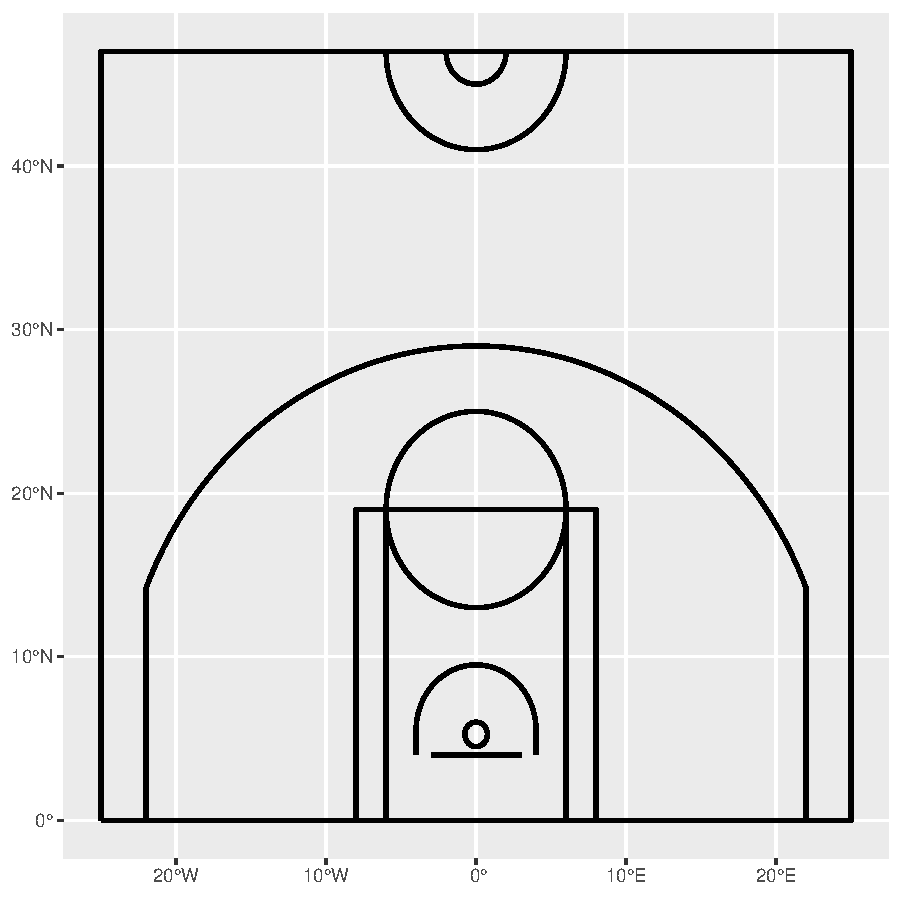
\includegraphics[width=.6\linewidth]{figure/Code-to-submit-Rnwauto-report-1} 

}


\begin{kframe}\begin{alltt}
\hlcom{# Load shots data}
\hlstd{shots_data} \hlkwb{<-} \hlkwd{data.table}\hlstd{()}
\hlkwa{for} \hlstd{(year} \hlkwa{in} \hlnum{2004}\hlopt{:}\hlnum{2005}\hlstd{) \{}

  \hlstd{file_name} \hlkwb{<-} \hlkwd{sprintf}\hlstd{(}\hlstr{"NBA_%d_Shots.csv"}\hlstd{, year)}
  \hlstd{year_data} \hlkwb{<-} \hlkwd{fread}\hlstd{(}\hlkwd{file.path}\hlstd{(DATA_DIR, file_name))}
  \hlstd{shots_data} \hlkwb{<-} \hlkwd{rbindlist}\hlstd{(}\hlkwd{list}\hlstd{(shots_data, year_data),} \hlkwc{use.names} \hlstd{=} \hlnum{TRUE}\hlstd{,} \hlkwc{fill} \hlstd{=} \hlnum{TRUE}\hlstd{)}

\hlstd{\}}

\hlcom{# Make SF point object}
\hlstd{shots_data_sf} \hlkwb{<-} \hlkwd{st_as_sf}\hlstd{(shots_data,} \hlkwc{coords} \hlstd{=} \hlkwd{c}\hlstd{(}\hlstr{"LOC_X"}\hlstd{,} \hlstr{"LOC_Y"}\hlstd{),} \hlkwc{crs} \hlstd{=} \hlkwd{st_crs}\hlstd{(half_court))}

\hlcom{## Identify shots in the restricted area}
\hlcom{################################################################################}

\hlcom{# The restricted area is currently just a semi circle, so we need to connect the}
\hlcom{# end points}
\hlstd{r_a} \hlkwb{<-} \hlstd{half_court} \hlopt
  \hlkwd{filter}\hlstd{(Feature}\hlopt{==}\hlstr{"Restricted area"}\hlstd{)}

\hlcom{# Create back line}
\hlstd{back_line} \hlkwb{<-} \hlkwd{st_sfc}\hlstd{(}\hlkwd{st_linestring}\hlstd{(}\hlkwd{matrix}\hlstd{(}\hlkwd{c}\hlstd{(}\hlopt{-}\hlnum{4}\hlstd{,} \hlnum{4}\hlstd{,} \hlnum{4}\hlstd{,} \hlnum{4}\hlstd{),} \hlkwc{ncol} \hlstd{=} \hlnum{2}\hlstd{,} \hlkwc{byrow} \hlstd{=} \hlnum{TRUE}\hlstd{)),} \hlkwc{crs} \hlstd{=} \hlkwd{st_crs}\hlstd{(r_a))}
\hlstd{r_a} \hlkwb{<-} \hlkwd{st_union}\hlstd{(r_a, back_line)} \hlcom{# Combine them}
\end{alltt}


{\ttfamily\noindent\color{warningcolor}{\#\# Warning: attribute variables are assumed to be spatially constant throughout all geometries}}\begin{alltt}
\hlcom{# Create polygon from coordinates}
\hlstd{r_a_coords} \hlkwb{<-} \hlkwd{st_coordinates}\hlstd{(r_a)} \hlcom{# Extract coordinates}
\hlstd{r_a_coords} \hlkwb{<-} \hlkwd{rbind}\hlstd{(r_a_coords, r_a_coords[}\hlnum{1}\hlstd{,])} \hlcom{# Make first and last the same}


\hlstd{r_a_polygon} \hlkwb{<-} \hlkwd{st_polygon}\hlstd{(}\hlkwd{list}\hlstd{(r_a_coords))} \hlcom{# Make polygon}
\hlstd{r_a_polygon} \hlkwb{<-} \hlkwd{st_zm}\hlstd{(r_a_polygon)} \hlcom{# Only keep x and y coords}
\hlstd{r_a_polygon} \hlkwb{<-} \hlkwd{st_make_valid}\hlstd{(r_a_polygon)}
\hlstd{r_a_polygon_sf} \hlkwb{<-} \hlkwd{st_sf}\hlstd{(}\hlkwc{geometry} \hlstd{=} \hlkwd{st_sfc}\hlstd{(r_a_polygon,} \hlkwc{crs} \hlstd{=} \hlkwd{st_crs}\hlstd{(r_a)))} \hlcom{# make sf object}

\hlcom{# Identify shots inside restricted area using st_within}
\hlstd{inside_r_a} \hlkwb{<-} \hlkwd{st_within}\hlstd{(shots_data_sf, r_a_polygon_sf)}
\end{alltt}


{\ttfamily\noindent\color{warningcolor}{\#\# Warning in st\_is\_longlat(x): bounding box has potentially an invalid value range for longlat data}}

{\ttfamily\noindent\color{warningcolor}{\#\# Warning in st\_is\_longlat(x): bounding box has potentially an invalid value range for longlat data}}\begin{alltt}
\hlcom{# Create_indicator}
\hlstd{shots_data_sf}\hlopt{$}\hlstd{inside_r_a} \hlkwb{<-} \hlkwd{as.integer}\hlstd{(}\hlkwd{lengths}\hlstd{(inside_r_a)} \hlopt{>} \hlnum{0}\hlstd{)}
\hlstd{shots_data}\hlopt{$}\hlstd{inside_r_a} \hlkwb{<-} \hlkwd{as.integer}\hlstd{(}\hlkwd{lengths}\hlstd{(inside_r_a)} \hlopt{>} \hlnum{0}\hlstd{)}


\hlcom{## Identify shots just behind the 3 point line}
\hlcom{################################################################################}


\hlcom{# HEAT MAP: per players}
\hlcom{################################################################################}
\hlcom{# Define a function to create the plot for a player}
\hlstd{create_player_plot} \hlkwb{<-} \hlkwa{function}\hlstd{(}\hlkwc{shots_data}\hlstd{,} \hlkwc{year}\hlstd{,} \hlkwc{player_name}\hlstd{) \{}

  \hlstd{data} \hlkwb{<-} \hlstd{shots_data} \hlopt
      \hlkwd{filter}\hlstd{(SEASON_1} \hlopt{==} \hlstd{year)} \hlopt
      \hlkwd{filter}\hlstd{(SHOT_MADE} \hlopt{==} \hlnum{TRUE}\hlstd{)} \hlopt
      \hlkwd{filter}\hlstd{(}\hlkwd{str_detect}\hlstd{(PLAYER_NAME, player_name))}

  \hlstd{title} \hlkwb{<-} \hlkwd{paste0}\hlstd{(player_name,} \hlstr{' - '}\hlstd{, year)}

  \hlkwd{ggplot}\hlstd{()} \hlopt{+}
    \hlkwd{geom_sf}\hlstd{(}\hlkwc{data} \hlstd{= half_court,} \hlkwc{color} \hlstd{=} \hlstr{"black"}\hlstd{,} \hlkwc{fill} \hlstd{=} \hlstr{"transparent"}\hlstd{,} \hlkwc{linewidth} \hlstd{=} \hlnum{1}\hlstd{)} \hlopt{+}
    \hlkwd{geom_point}\hlstd{(}\hlkwc{data} \hlstd{= data,} \hlkwd{aes}\hlstd{(}\hlkwc{x} \hlstd{= LOC_X,} \hlkwc{y} \hlstd{= LOC_Y),}
               \hlkwc{size} \hlstd{=} \hlnum{1}\hlstd{,} \hlkwc{alpha} \hlstd{=} \hlnum{0.1}\hlstd{)} \hlopt{+}
    \hlkwd{geom_density_2d_filled}\hlstd{(data,} \hlkwc{mapping} \hlstd{=} \hlkwd{aes}\hlstd{(}\hlkwc{x} \hlstd{= LOC_X,} \hlkwc{y} \hlstd{= LOC_Y,} \hlkwc{fill} \hlstd{= ..level..),}
                           \hlkwc{contour_var} \hlstd{=} \hlstr{"ndensity"}\hlstd{,} \hlkwc{breaks} \hlstd{=} \hlkwd{seq}\hlstd{(}\hlnum{0.03}\hlstd{,} \hlnum{1.0}\hlstd{,} \hlkwc{length.out} \hlstd{=} \hlnum{80}\hlstd{),} \hlkwc{alpha} \hlstd{=} \hlnum{.7}\hlstd{)} \hlopt{+}
    \hlkwd{scale_x_continuous}\hlstd{(}\hlkwc{limits} \hlstd{=} \hlkwd{c}\hlstd{(}\hlopt{-}\hlnum{27.5}\hlstd{,} \hlnum{27.5}\hlstd{))} \hlopt{+}
    \hlkwd{scale_y_continuous}\hlstd{(}\hlkwc{limits} \hlstd{=} \hlkwd{c}\hlstd{(}\hlnum{0}\hlstd{,} \hlnum{45}\hlstd{))} \hlopt{+}
    \hlkwd{labs}\hlstd{(}\hlkwc{title} \hlstd{= title)} \hlopt{+}
    \hlkwd{theme}\hlstd{(}\hlkwc{legend.position} \hlstd{=} \hlstr{"none"}\hlstd{,}
          \hlkwc{plot.title} \hlstd{=} \hlkwd{element_text}\hlstd{(}\hlkwc{hjust} \hlstd{=} \hlnum{0.5}\hlstd{,} \hlkwc{size} \hlstd{=} \hlnum{20}\hlstd{),}
          \hlkwc{axis.title.x} \hlstd{=} \hlkwd{element_blank}\hlstd{(),}
          \hlkwc{axis.title.y} \hlstd{=} \hlkwd{element_blank}\hlstd{(),}
          \hlkwc{axis.text.x} \hlstd{=} \hlkwd{element_blank}\hlstd{(),}
          \hlkwc{axis.text.y} \hlstd{=} \hlkwd{element_blank}\hlstd{(),}
          \hlkwc{axis.ticks} \hlstd{=} \hlkwd{element_blank}\hlstd{(),}
          \hlkwc{panel.grid.major} \hlstd{=} \hlkwd{element_blank}\hlstd{(),}
          \hlkwc{panel.grid.minor} \hlstd{=} \hlkwd{element_blank}\hlstd{(),}
          \hlkwc{panel.background} \hlstd{=} \hlkwd{element_blank}\hlstd{())}
\hlstd{\}}

\hlcom{# Create plots for each player}
\hlstd{player1} \hlkwb{<-} \hlkwd{create_player_plot}\hlstd{(shots_data,} \hlnum{2013}\hlstd{,} \hlstr{"LeBron James"}\hlstd{)}
\hlstd{player2} \hlkwb{<-} \hlkwd{create_player_plot}\hlstd{(shots_data,} \hlnum{2016}\hlstd{,} \hlstr{"Stephen Curry"}\hlstd{)}
\hlstd{player3} \hlkwb{<-} \hlkwd{create_player_plot}\hlstd{(shots_data,} \hlnum{2019}\hlstd{,} \hlstr{"Giannis Antetokounmpo"}\hlstd{)}

\hlcom{# Arrange plots side by side}
\hlstd{side_by_side_plots} \hlkwb{<-} \hlkwd{grid.arrange}\hlstd{(player1, player2, player3,} \hlkwc{ncol} \hlstd{=} \hlnum{3}\hlstd{)}
\end{alltt}


{\ttfamily\noindent\color{warningcolor}{\#\# Warning: The dot-dot notation (`..level..`) was deprecated in ggplot2 3.4.0.\\\#\# i Please use `after\_stat(level)` instead.\\\#\# This warning is displayed once every 8 hours.\\\#\# Call `lifecycle::last\_lifecycle\_warnings()` to see where this warning was generated.}}\end{kframe}

{\centering 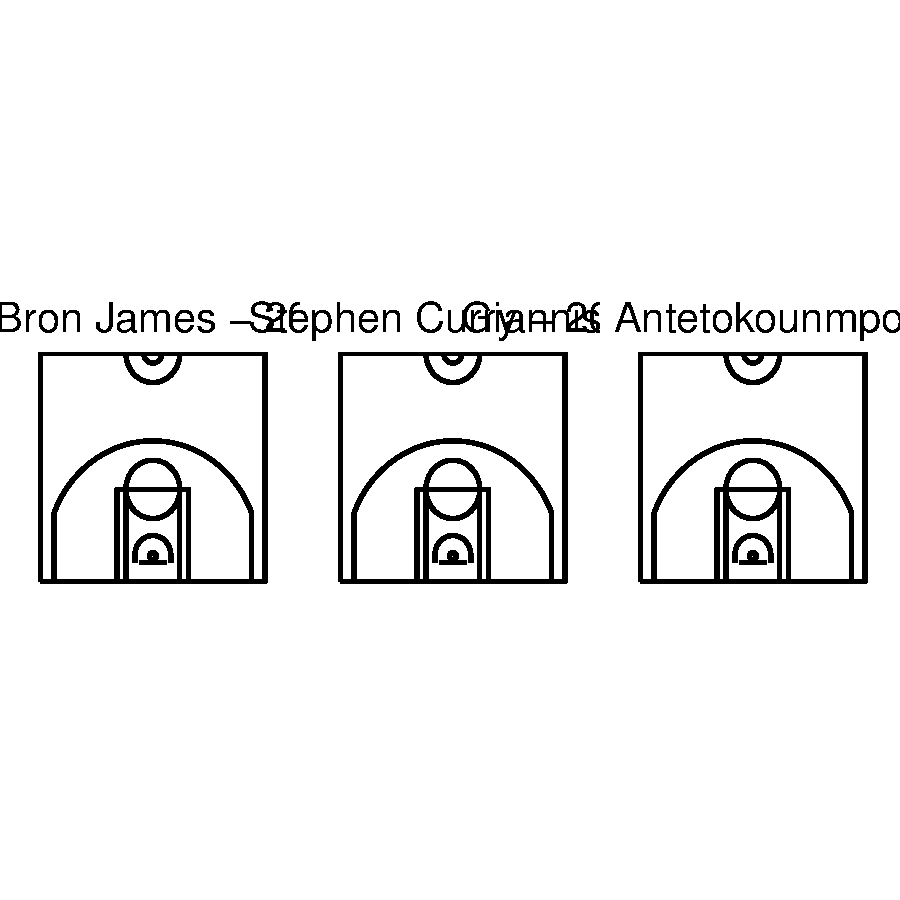
\includegraphics[width=.6\linewidth]{figure/Code-to-submit-Rnwauto-report-2} 

}


\begin{kframe}\begin{alltt}
\hlkwd{print}\hlstd{(side_by_side_plots)}
\end{alltt}
\begin{verbatim}
## TableGrob (1 x 3) "arrange": 3 grobs
##   z     cells    name           grob
## 1 1 (1-1,1-1) arrange gtable[layout]
## 2 2 (1-1,2-2) arrange gtable[layout]
## 3 3 (1-1,3-3) arrange gtable[layout]
\end{verbatim}
\begin{alltt}
\hlcom{# HEAT MAP:  overall}
\hlcom{################################################################################}
\hlstd{outside_before} \hlkwb{<-} \hlstd{shots_data} \hlopt
  \hlkwd{filter}\hlstd{(SEASON_1} \hlopt{==} \hlnum{2004}\hlstd{)} \hlopt
  \hlkwd{filter}\hlstd{(BASIC_ZONE} \hlopt{!=} \hlstr{"Restricted Area"}\hlstd{)}

\hlstd{outside_now} \hlkwb{<-} \hlstd{shots_data} \hlopt
  \hlkwd{filter}\hlstd{(SEASON_1} \hlopt{==} \hlnum{2019}\hlstd{)} \hlopt
  \hlkwd{filter}\hlstd{(BASIC_ZONE} \hlopt{!=} \hlstr{"Restricted Area"}\hlstd{)}

\hlstd{before} \hlkwb{<-} \hlkwd{ggplot}\hlstd{()} \hlopt{+}
  \hlkwd{geom_sf}\hlstd{(}\hlkwc{data} \hlstd{= half_court,} \hlkwc{color} \hlstd{=} \hlstr{"black"}\hlstd{,} \hlkwc{fill} \hlstd{=} \hlstr{"transparent"}\hlstd{,} \hlkwc{linewidth} \hlstd{=} \hlnum{1}\hlstd{)} \hlopt{+}
  \hlkwd{geom_density_2d_filled}\hlstd{(outside_before,} \hlkwc{mapping} \hlstd{=} \hlkwd{aes}\hlstd{(}\hlkwc{x} \hlstd{= LOC_X,} \hlkwc{y} \hlstd{= LOC_Y,} \hlkwc{fill} \hlstd{= ..level..),}
                         \hlkwc{contour_var} \hlstd{=} \hlstr{"ndensity"}\hlstd{,} \hlkwc{breaks} \hlstd{=} \hlkwd{seq}\hlstd{(}\hlnum{0.1}\hlstd{,} \hlnum{1.0}\hlstd{,} \hlkwc{length.out} \hlstd{=} \hlnum{50}\hlstd{),} \hlkwc{alpha} \hlstd{=} \hlnum{.8}\hlstd{)} \hlopt{+}
  \hlkwd{scale_x_continuous}\hlstd{(}\hlkwc{limits} \hlstd{=} \hlkwd{c}\hlstd{(}\hlopt{-}\hlnum{27.5}\hlstd{,} \hlnum{27.5}\hlstd{))} \hlopt{+}
  \hlkwd{scale_y_continuous}\hlstd{(}\hlkwc{limits} \hlstd{=} \hlkwd{c}\hlstd{(}\hlnum{0}\hlstd{,} \hlnum{45}\hlstd{))} \hlopt{+}
  \hlkwd{labs}\hlstd{(}\hlkwc{title} \hlstd{=} \hlstr{'Shots attempts 2004'}\hlstd{)} \hlopt{+}
  \hlkwd{theme}\hlstd{(}\hlkwc{legend.position} \hlstd{=} \hlstr{"none"}\hlstd{,}
        \hlkwc{plot.title} \hlstd{=} \hlkwd{element_text}\hlstd{(}\hlkwc{hjust} \hlstd{=} \hlnum{0.5}\hlstd{,} \hlkwc{size} \hlstd{=} \hlnum{20}\hlstd{),}
        \hlkwc{axis.title.x} \hlstd{=} \hlkwd{element_blank}\hlstd{(),}
        \hlkwc{axis.title.y} \hlstd{=} \hlkwd{element_blank}\hlstd{(),}
        \hlkwc{axis.text.x} \hlstd{=} \hlkwd{element_blank}\hlstd{(),}
        \hlkwc{axis.text.y} \hlstd{=} \hlkwd{element_blank}\hlstd{(),}
        \hlkwc{axis.ticks} \hlstd{=} \hlkwd{element_blank}\hlstd{(),}
        \hlkwc{panel.grid.major} \hlstd{=} \hlkwd{element_blank}\hlstd{(),}
        \hlkwc{panel.grid.minor} \hlstd{=} \hlkwd{element_blank}\hlstd{(),}
        \hlkwc{panel.background} \hlstd{=} \hlkwd{element_blank}\hlstd{())}

\hlstd{now} \hlkwb{<-} \hlkwd{ggplot}\hlstd{()} \hlopt{+}
  \hlkwd{geom_sf}\hlstd{(}\hlkwc{data} \hlstd{= half_court,} \hlkwc{color} \hlstd{=} \hlstr{"black"}\hlstd{,} \hlkwc{fill} \hlstd{=} \hlstr{"transparent"}\hlstd{,} \hlkwc{linewidth} \hlstd{=} \hlnum{1}\hlstd{)} \hlopt{+}
  \hlkwd{geom_density_2d_filled}\hlstd{(outside_now,} \hlkwc{mapping} \hlstd{=} \hlkwd{aes}\hlstd{(}\hlkwc{x} \hlstd{= LOC_X,} \hlkwc{y} \hlstd{= LOC_Y,} \hlkwc{fill} \hlstd{= ..level..),}
                         \hlkwc{contour_var} \hlstd{=} \hlstr{"ndensity"}\hlstd{,} \hlkwc{breaks} \hlstd{=} \hlkwd{seq}\hlstd{(}\hlnum{0.1}\hlstd{,} \hlnum{1.0}\hlstd{,} \hlkwc{length.out} \hlstd{=} \hlnum{50}\hlstd{),} \hlkwc{alpha} \hlstd{=} \hlnum{.8}\hlstd{)} \hlopt{+}
  \hlkwd{scale_x_continuous}\hlstd{(}\hlkwc{limits} \hlstd{=} \hlkwd{c}\hlstd{(}\hlopt{-}\hlnum{27.5}\hlstd{,} \hlnum{27.5}\hlstd{))} \hlopt{+}
  \hlkwd{scale_y_continuous}\hlstd{(}\hlkwc{limits} \hlstd{=} \hlkwd{c}\hlstd{(}\hlnum{0}\hlstd{,} \hlnum{45}\hlstd{))} \hlopt{+}
  \hlkwd{labs}\hlstd{(}\hlkwc{title} \hlstd{=} \hlstr{'Shots attempts 2019'}\hlstd{)} \hlopt{+}
  \hlkwd{theme}\hlstd{(}\hlkwc{legend.position} \hlstd{=} \hlstr{"none"}\hlstd{,}
        \hlkwc{plot.title} \hlstd{=} \hlkwd{element_text}\hlstd{(}\hlkwc{hjust} \hlstd{=} \hlnum{0.5}\hlstd{,} \hlkwc{size} \hlstd{=} \hlnum{20}\hlstd{),}
        \hlkwc{axis.title.x} \hlstd{=} \hlkwd{element_blank}\hlstd{(),}
        \hlkwc{axis.title.y} \hlstd{=} \hlkwd{element_blank}\hlstd{(),}
        \hlkwc{axis.text.x} \hlstd{=} \hlkwd{element_blank}\hlstd{(),}
        \hlkwc{axis.text.y} \hlstd{=} \hlkwd{element_blank}\hlstd{(),}
        \hlkwc{axis.ticks} \hlstd{=} \hlkwd{element_blank}\hlstd{(),}
        \hlkwc{panel.grid.major} \hlstd{=} \hlkwd{element_blank}\hlstd{(),}
        \hlkwc{panel.grid.minor} \hlstd{=} \hlkwd{element_blank}\hlstd{(),}
        \hlkwc{panel.background} \hlstd{=} \hlkwd{element_blank}\hlstd{())}

\hlstd{side_by_side_plots} \hlkwb{<-} \hlkwd{grid.arrange}\hlstd{(before, now,} \hlkwc{ncol} \hlstd{=} \hlnum{2}\hlstd{)}
\end{alltt}


{\ttfamily\noindent\color{warningcolor}{\#\# Warning: Removed 445 rows containing non-finite outside the scale range\\\#\# (`stat\_density2d\_filled()`).}}\end{kframe}

{\centering 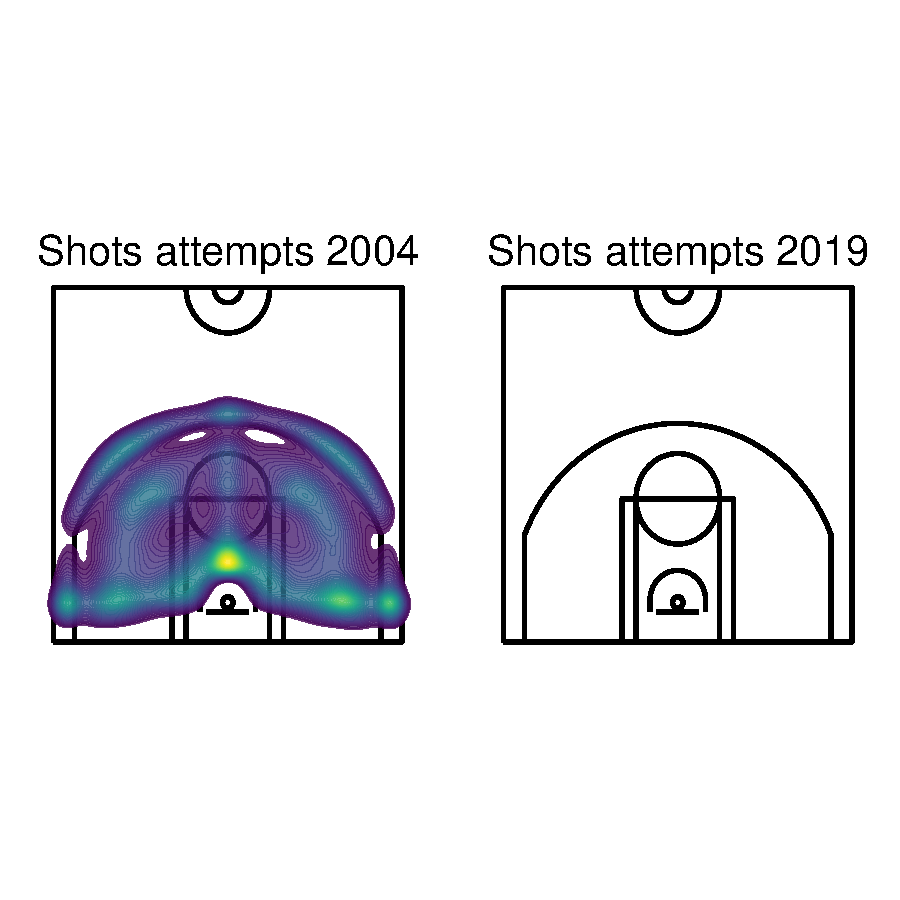
\includegraphics[width=.6\linewidth]{figure/Code-to-submit-Rnwauto-report-3} 

}


\begin{kframe}\begin{alltt}
\hlkwd{print}\hlstd{(side_by_side_plots)}
\end{alltt}
\begin{verbatim}
## TableGrob (1 x 2) "arrange": 2 grobs
##   z     cells    name           grob
## 1 1 (1-1,1-1) arrange gtable[layout]
## 2 2 (1-1,2-2) arrange gtable[layout]
\end{verbatim}
\begin{alltt}
\hlcom{# ACCEPTANCE RATE:  Curry}
\hlcom{################################################################################}
\hlstd{shots_curry} \hlkwb{<-} \hlstd{shots_data} \hlopt
  \hlkwd{filter}\hlstd{(SEASON_1} \hlopt{==} \hlnum{2016}\hlstd{)} \hlopt
  \hlkwd{filter}\hlstd{(}\hlkwd{str_detect}\hlstd{(PLAYER_NAME,} \hlstr{"Stephen Curry"}\hlstd{))} \hlopt
  \hlkwd{select}\hlstd{(PLAYER_NAME, GAME_DATE, EVENT_TYPE, SHOT_MADE, SHOT_TYPE, LOC_X, LOC_Y)}

\hlstd{shots_curry}
\end{alltt}
\begin{verbatim}
## Empty data.table (0 rows and 7 cols): PLAYER_NAME,GAME_DATE,EVENT_TYPE,SHOT_MADE,SHOT_TYPE,LOC_X...
\end{verbatim}
\begin{alltt}
\hlcom{# Create scatter plot}
\hlstd{scatter_plot} \hlkwb{<-} \hlkwd{ggplot}\hlstd{()} \hlopt{+}
  \hlkwd{geom_sf}\hlstd{(}\hlkwc{data} \hlstd{= half_court,} \hlkwc{color} \hlstd{=} \hlstr{"black"}\hlstd{,} \hlkwc{fill} \hlstd{=} \hlstr{"transparent"}\hlstd{,} \hlkwc{linewidth} \hlstd{=} \hlnum{1}\hlstd{)} \hlopt{+}
  \hlkwd{geom_point}\hlstd{(}\hlkwc{data} \hlstd{= shots_curry,} \hlkwd{aes}\hlstd{(}\hlkwc{x} \hlstd{= LOC_X,} \hlkwc{y} \hlstd{= LOC_Y,} \hlkwc{color} \hlstd{= SHOT_MADE),} \hlkwc{alpha} \hlstd{=} \hlnum{0.3}\hlstd{)} \hlopt{+}  \hlcom{# Add points with transparency}
  \hlkwd{labs}\hlstd{(}\hlkwc{title} \hlstd{=} \hlstr{"Shots Scatterplot"}\hlstd{,} \hlkwc{x} \hlstd{=} \hlstr{"LOC_X"}\hlstd{,} \hlkwc{y} \hlstd{=} \hlstr{"LOC_Y"}\hlstd{)} \hlopt{+}  \hlcom{# Add title and axis labels}
  \hlkwd{theme_minimal}\hlstd{()} \hlopt{+}
  \hlkwd{scale_x_continuous}\hlstd{(}\hlkwc{limits} \hlstd{=} \hlkwd{c}\hlstd{(}\hlopt{-}\hlnum{27.5}\hlstd{,} \hlnum{27.5}\hlstd{))} \hlopt{+}
  \hlkwd{scale_y_continuous}\hlstd{(}\hlkwc{limits} \hlstd{=} \hlkwd{c}\hlstd{(}\hlnum{0}\hlstd{,} \hlnum{45}\hlstd{))} \hlopt{+}
  \hlkwd{labs}\hlstd{(}\hlkwc{title} \hlstd{=} \hlstr{'Stephen Curry 2016 shots'}\hlstd{)} \hlopt{+}
  \hlkwd{theme}\hlstd{(}\hlkwc{legend.position} \hlstd{=} \hlstr{"bottom"}\hlstd{,}
        \hlkwc{plot.title} \hlstd{=} \hlkwd{element_text}\hlstd{(}\hlkwc{hjust} \hlstd{=} \hlnum{0.5}\hlstd{,} \hlkwc{size} \hlstd{=} \hlnum{20}\hlstd{),}
        \hlkwc{axis.title.x} \hlstd{=} \hlkwd{element_blank}\hlstd{(),}
        \hlkwc{axis.title.y} \hlstd{=} \hlkwd{element_blank}\hlstd{(),}
        \hlkwc{axis.text.x} \hlstd{=} \hlkwd{element_blank}\hlstd{(),}
        \hlkwc{axis.text.y} \hlstd{=} \hlkwd{element_blank}\hlstd{(),}
        \hlkwc{axis.ticks} \hlstd{=} \hlkwd{element_blank}\hlstd{(),}
        \hlkwc{panel.grid.major} \hlstd{=} \hlkwd{element_blank}\hlstd{(),}
        \hlkwc{panel.grid.minor} \hlstd{=} \hlkwd{element_blank}\hlstd{(),}
        \hlkwc{panel.background} \hlstd{=} \hlkwd{element_blank}\hlstd{())}

\hlcom{# Print the scatter plot}
\hlkwd{print}\hlstd{(scatter_plot)}
\end{alltt}
\end{kframe}

{\centering 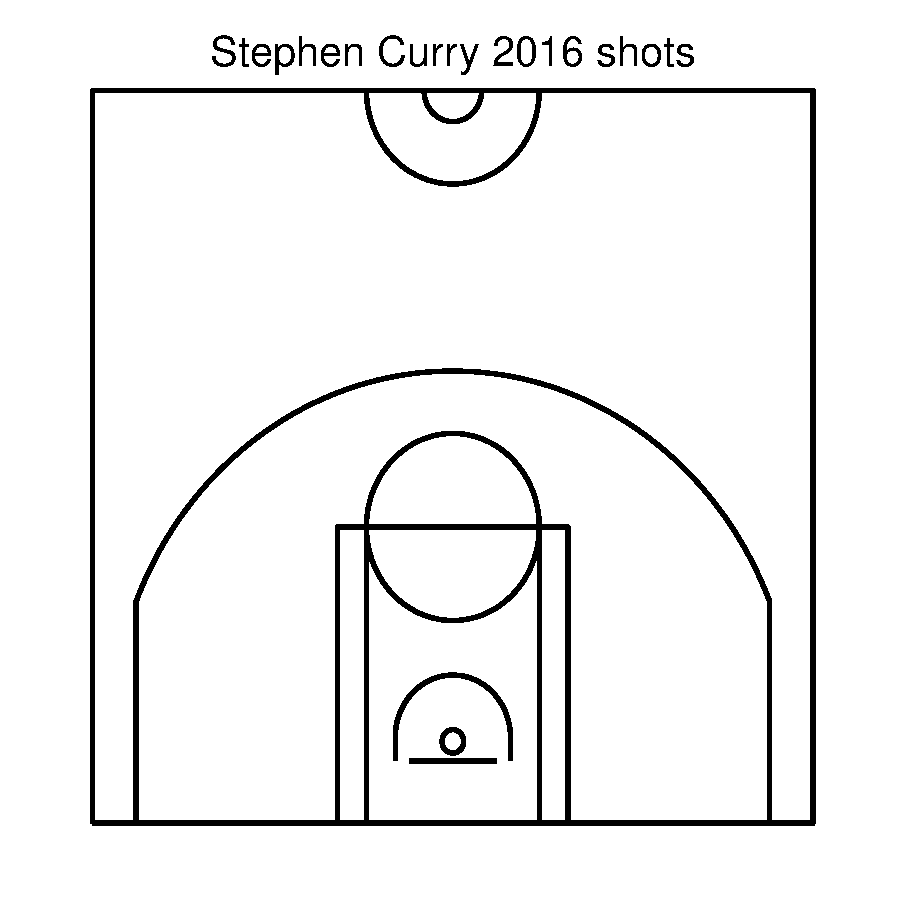
\includegraphics[width=.6\linewidth]{figure/Code-to-submit-Rnwauto-report-4} 

}


\begin{kframe}\begin{alltt}
\hlstd{shots_data}\hlopt{$}\hlstd{LOC_X_simple} \hlkwb{<-} \hlkwd{as.integer}\hlstd{(shots_data}\hlopt{$}\hlstd{LOC_X}\hlopt{/}\hlnum{4}\hlstd{)}\hlopt{*}\hlnum{4}
\hlstd{shots_data}\hlopt{$}\hlstd{LOC_Y_simple} \hlkwb{<-} \hlkwd{as.integer}\hlstd{(shots_data}\hlopt{$}\hlstd{LOC_Y}\hlopt{/}\hlnum{4}\hlstd{)}\hlopt{*}\hlnum{4}

\hlstd{shot_summary} \hlkwb{<-} \hlstd{shots_data} \hlopt
  \hlkwd{group_by}\hlstd{(LOC_X_simple, LOC_Y_simple)} \hlopt
  \hlkwd{summarize}\hlstd{(}\hlkwc{total_shots} \hlstd{=} \hlkwd{n}\hlstd{(),} \hlkwc{made_shots} \hlstd{=} \hlkwd{sum}\hlstd{(SHOT_MADE))}
\end{alltt}


{\ttfamily\noindent\itshape\color{messagecolor}{\#\# `summarise()` has grouped output by 'LOC\_X\_simple'. You can override using the `.groups`\\\#\# argument.}}\begin{alltt}
\hlcom{# Calculate the acceptance rate}
\hlstd{shot_summary}\hlopt{$}\hlstd{acceptance_rate} \hlkwb{<-} \hlstd{shot_summary}\hlopt{$}\hlstd{made_shots} \hlopt{/} \hlstd{shot_summary}\hlopt{$}\hlstd{total_shots} \hlopt{*} \hlnum{100}

\hlcom{# Create the heatmap plot}
\hlstd{heatmap_plot} \hlkwb{<-} \hlkwd{ggplot}\hlstd{()} \hlopt{+}
  \hlkwd{geom_sf}\hlstd{(}\hlkwc{data} \hlstd{= half_court,} \hlkwc{color} \hlstd{=} \hlstr{"grey"}\hlstd{,} \hlkwc{fill} \hlstd{=} \hlstr{"transparent"}\hlstd{,} \hlkwc{linewidth} \hlstd{=} \hlnum{1}\hlstd{,} \hlkwc{alpha}\hlstd{=}\hlnum{0.8}\hlstd{)} \hlopt{+}  \hlcom{# Plot the basketball court}
  \hlkwd{geom_raster}\hlstd{(}\hlkwc{data} \hlstd{= shot_summary,} \hlkwd{aes}\hlstd{(}\hlkwc{x} \hlstd{= LOC_X_simple,} \hlkwc{y} \hlstd{= LOC_Y_simple,} \hlkwc{fill} \hlstd{= acceptance_rate),} \hlkwc{alpha}\hlstd{=}\hlnum{0.5}\hlstd{)} \hlopt{+}
  \hlkwd{scale_fill_gradient}\hlstd{(}\hlkwc{low} \hlstd{=} \hlstr{"red"}\hlstd{,} \hlkwc{high} \hlstd{=} \hlstr{"darkblue"}\hlstd{,} \hlkwc{name} \hlstd{=} \hlstr{"Acceptance Rate"}\hlstd{)} \hlopt{+}  \hlcom{# Customize fill color scale}
  \hlkwd{scale_x_continuous}\hlstd{(}\hlkwc{limits} \hlstd{=} \hlkwd{c}\hlstd{(}\hlopt{-}\hlnum{27.5}\hlstd{,} \hlnum{27.5}\hlstd{))} \hlopt{+}  \hlcom{# Set x-axis limits}
  \hlkwd{scale_y_continuous}\hlstd{(}\hlkwc{limits} \hlstd{=} \hlkwd{c}\hlstd{(}\hlnum{0}\hlstd{,} \hlnum{45}\hlstd{))} \hlopt{+}  \hlcom{# Set y-axis limits}
  \hlkwd{labs}\hlstd{(}\hlkwc{title} \hlstd{=} \hlstr{"Shooting Percentage Heatmap"}\hlstd{)} \hlopt{+}  \hlcom{# Add title}
  \hlkwd{theme_minimal}\hlstd{()} \hlopt{+}
  \hlkwd{theme}\hlstd{(}\hlkwc{legend.position} \hlstd{=} \hlstr{"bottom"}\hlstd{,}
        \hlkwc{plot.title} \hlstd{=} \hlkwd{element_text}\hlstd{(}\hlkwc{hjust} \hlstd{=} \hlnum{0.5}\hlstd{,} \hlkwc{size} \hlstd{=} \hlnum{20}\hlstd{),}
        \hlkwc{axis.title.x} \hlstd{=} \hlkwd{element_blank}\hlstd{(),}
        \hlkwc{axis.title.y} \hlstd{=} \hlkwd{element_blank}\hlstd{(),}
        \hlkwc{axis.text.x} \hlstd{=} \hlkwd{element_blank}\hlstd{(),}
        \hlkwc{axis.text.y} \hlstd{=} \hlkwd{element_blank}\hlstd{(),}
        \hlkwc{axis.ticks} \hlstd{=} \hlkwd{element_blank}\hlstd{(),}
        \hlkwc{panel.grid.major} \hlstd{=} \hlkwd{element_blank}\hlstd{(),}
        \hlkwc{panel.grid.minor} \hlstd{=} \hlkwd{element_blank}\hlstd{(),}
        \hlkwc{panel.background} \hlstd{=} \hlkwd{element_blank}\hlstd{())}

\hlcom{# Print the heatmap plot}
\hlkwd{print}\hlstd{(heatmap_plot)}
\end{alltt}


{\ttfamily\noindent\color{warningcolor}{\#\# Warning: Removed 132 rows containing missing values or values outside the scale range\\\#\# (`geom\_raster()`).}}\end{kframe}

{\centering 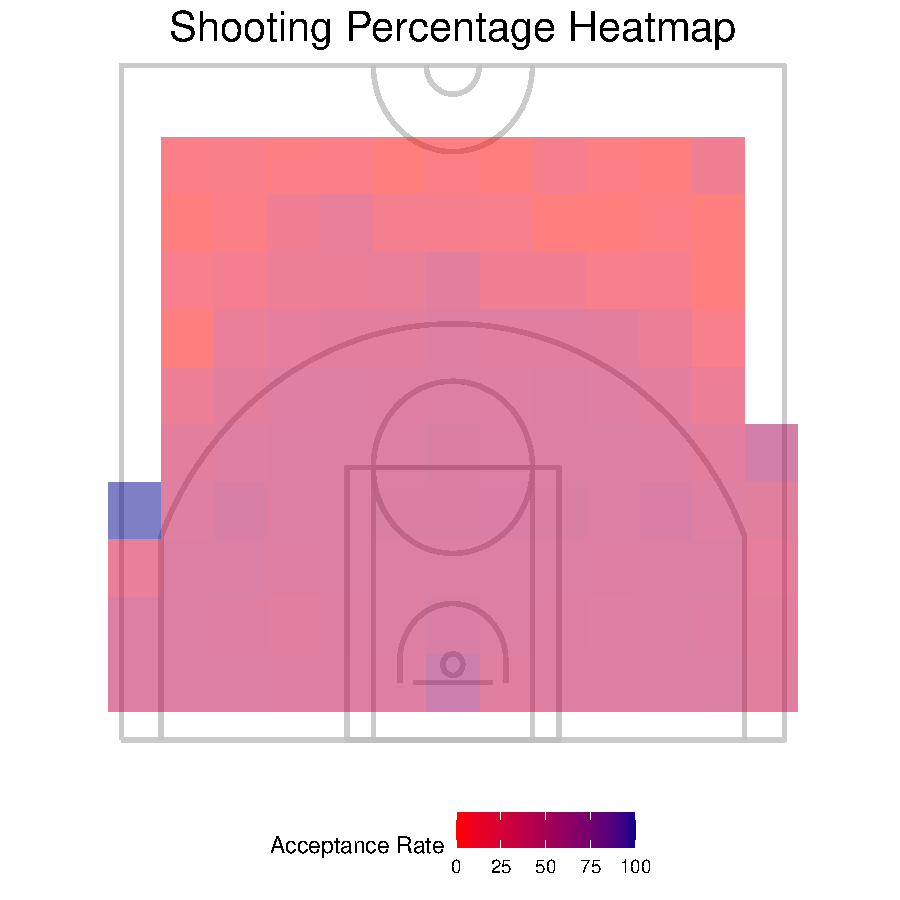
\includegraphics[width=.6\linewidth]{figure/Code-to-submit-Rnwauto-report-5} 

}


\begin{kframe}\begin{alltt}
\hlstd{side_by_side_plots} \hlkwb{<-} \hlkwd{grid.arrange}\hlstd{(scatter_plot, heatmap_plot,} \hlkwc{ncol} \hlstd{=} \hlnum{2}\hlstd{)}
\end{alltt}


{\ttfamily\noindent\color{warningcolor}{\#\# Warning: Removed 132 rows containing missing values or values outside the scale range\\\#\# (`geom\_raster()`).}}\end{kframe}

{\centering 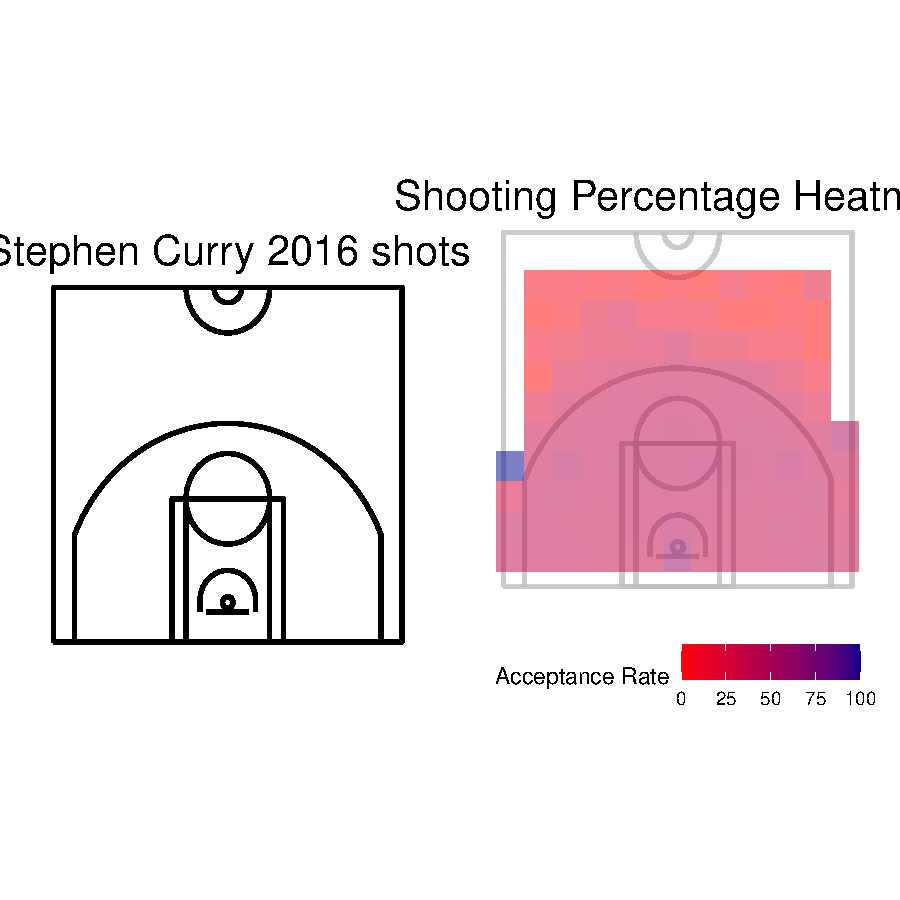
\includegraphics[width=.6\linewidth]{figure/Code-to-submit-Rnwauto-report-6} 

}


\begin{kframe}\begin{alltt}
\hlkwd{print}\hlstd{(side_by_side_plots)}
\end{alltt}
\begin{verbatim}
## TableGrob (1 x 2) "arrange": 2 grobs
##   z     cells    name           grob
## 1 1 (1-1,1-1) arrange gtable[layout]
## 2 2 (1-1,2-2) arrange gtable[layout]
\end{verbatim}
\end{kframe}
\end{knitrout}

The R session information (including the OS info, R version and all
packages used):

\begin{knitrout}
\definecolor{shadecolor}{rgb}{0.969, 0.969, 0.969}\color{fgcolor}\begin{kframe}
\begin{alltt}
\hlkwd{sessionInfo}\hlstd{()}
\end{alltt}
\begin{verbatim}
## R version 4.3.1 (2023-06-16)
## Platform: aarch64-apple-darwin20 (64-bit)
## Running under: macOS Sonoma 14.0
## 
## Matrix products: default
## BLAS:   /System/Library/Frameworks/Accelerate.framework/Versions/A/Frameworks/vecLib.framework/Versions/A/libBLAS.dylib 
## LAPACK: /Library/Frameworks/R.framework/Versions/4.3-arm64/Resources/lib/libRlapack.dylib;  LAPACK version 3.11.0
## 
## locale:
## [1] en_US.UTF-8/en_US.UTF-8/en_US.UTF-8/C/en_US.UTF-8/en_US.UTF-8
## 
## time zone: Europe/Rome
## tzcode source: internal
## 
## attached base packages:
## [1] stats     graphics  grDevices utils     datasets  methods   base     
## 
## other attached packages:
##  [1] gridExtra_2.3     lubridate_1.9.3   stringr_1.5.1     paletteer_1.6.0  
##  [5] ggplot2_3.5.0     sf_1.0-15         progress_1.2.3    dplyr_1.1.4      
##  [9] jsonlite_1.8.8    data.table_1.15.2
## 
## loaded via a namespace (and not attached):
##  [1] s2_1.1.6           utf8_1.2.4         generics_0.1.3     class_7.3-22      
##  [5] KernSmooth_2.23-22 stringi_1.8.3      hms_1.1.3          magrittr_2.0.3    
##  [9] evaluate_0.23      grid_4.3.1         timechange_0.3.0   e1071_1.7-14      
## [13] DBI_1.2.2          rematch2_2.1.2     fansi_1.0.6        viridisLite_0.4.2 
## [17] scales_1.3.0       isoband_0.2.7      cli_3.6.2          rlang_1.1.3       
## [21] crayon_1.5.2       units_0.8-5        munsell_0.5.0      withr_3.0.0       
## [25] tools_4.3.1        colorspace_2.1-0   vctrs_0.6.5        R6_2.5.1          
## [29] proxy_0.4-27       lifecycle_1.0.4    classInt_0.4-10    MASS_7.3-60.0.1   
## [33] pkgconfig_2.0.3    pillar_1.9.0       gtable_0.3.4       glue_1.7.0        
## [37] Rcpp_1.0.12        xfun_0.42          tibble_3.2.1       tidyselect_1.2.1  
## [41] highr_0.10         rstudioapi_0.15.0  knitr_1.45         farver_2.1.1      
## [45] labeling_0.4.3     wk_0.9.1           compiler_4.3.1     prettyunits_1.2.0
\end{verbatim}
\begin{alltt}
\hlkwd{Sys.time}\hlstd{()}
\end{alltt}
\begin{verbatim}
## [1] "2024-03-27 12:16:49 CET"
\end{verbatim}
\end{kframe}
\end{knitrout}


\end{document}
